% =============================================================================
% 4. PROPOSED METHODOLOGY: BIODINO-EDGE
% =============================================================================
\section{Proposed Methodology: BioDINO-Edge}
\label{sec:methodology}
Building upon the theoretical framework and operational constraints established in Section~\ref{sec:problem_formulation}, BioDINO-Edge addresses few-shot plant disease diagnosis through closed-form discriminative projection over frozen foundation representations, paired with an uncertainty-gated cascaded inference pipeline for resource-constrained edge hardware.

\subsection{Pipeline Overview}
\label{sec:system_architecture}
BioDINO-Edge splits its workflow into an offline analytical calibration phase (Phase~0) and an adaptive two-tier runtime cascade (Phase~1), as shown in Fig.~\ref{fig:architecture}. In Phase~0, a small support set ($K = 5$ labeled leaves per class) is expanded with multi-view augmentation. Features from the frozen DINOv2 and BioCLIP backbones are then used to compute Tier-1 visual prototypes and regularized Fisher-LDA projection weights in closed form, while botanical text prototypes are pre-encoded and cached. At inference (Phase~1), each query first goes through the lightweight Tier-1 DINOv2 encoder. An uncertainty gate lets clear leaves exit immediately and escalates only ambiguous queries to the deeper Tier-2 multimodal stage. High-confidence predictions can then update the Tier-2 projections through background transductive recalibration. Table~\ref{tab:notation} summarizes the mathematical notations and descriptions used across the framework.

\begin{table*}[htbp]
\caption{Summary of mathematical notations and descriptions used in BioDINO-Edge.}
\label{tab:notation}
\centering
\footnotesize
\begin{tabularx}{\textwidth}{lX}
\toprule
\textbf{Notation} & \textbf{Mathematical Description and Operational Meaning} \\
\midrule
$C, K, N_s$ & Number of pathology classes, shots per class ($K=5$), and total support size ($N_s = C \cdot K$). \\
$\phi_{\text{dino}}(\cdot), \phi_{\text{bio}}(\cdot)$ & Frozen INT8 DINOv2-Small ($d_1 = 384$) and BioCLIP ViT-B/16 ($d_2 = 512$) encoders. \\
$\mathbf{z} \in \mathbb{R}^{896}$ & Concatenated joint foliar descriptor: $\mathbf{z} = [\mathbf{f}_{\text{bio}} \,\|\, \mathbf{f}_{\text{dino}}] \in \mathbb{R}^{896}$. \\
$\mathbf{P}_{\text{dino}}, \mathbf{P}_{\text{text}}$ & Tier-1 visual prototypes ($\mathbb{R}^{C \times 384}$) and cached botanical text prototypes ($\mathbb{R}^{C \times 512}$). \\
$\mathbf{S}_W, \hat{\mathbf{\Sigma}}$ & Empirical pooled within-class scatter matrix and Ledoit--Wolf regularized covariance matrix. \\
$\rho^*, \nu$ & Analytical shrinkage intensity factor $\rho^* \in (0, 1]$ and mean trace shrinkage target $\nu = \frac{1}{d}\text{Tr}(\mathbf{S}_W)$. \\
$\mathbf{W}, \mathbf{b}$ & Fisher-LDA discriminant projection matrix ($\mathbb{R}^{C \times 896}$) and class bias vector ($\mathbb{R}^C$). \\
$\mathcal{C}(\mathbf{x}), \tau_{\text{conf}}$ & Dual-metric uncertainty gate (Shannon entropy and top-2 margin) and escalation threshold ($\tau_{\text{conf}} = 0.35$). \\
$w_{\text{lda}}$ & Multimodal consensus blending weight ($w_{\text{lda}} = 0.75$, weighting visual Fisher against text posteriors). \\
$\gamma$ & Inverse temperature logit scaling parameter ($\gamma = 20.0$). \\
$\mathcal{Q}_{\text{anchor}}^{(c)}$ & High-confidence streaming query buffer ($\max_c p_c \ge 0.70$) for background transductive recalibration. \\
$\epsilon_{\text{esc}}, \text{FNR}$ & Agronomic disease escape bound ($\epsilon_{\text{esc}} = 1.0\%$) and false-negative disease rate. \\
$L_{\max}, \overline{L}_{\text{inf}}$ & Real-time per-frame latency budget ($L_{\max} = 170$\,ms) and mean cascading stream latency. \\
$T_{\max}, T_{\text{adapt}}$ & Sub-second on-device adaptation budget ($T_{\max} = 1.0$\,s) and novel-pathology registration latency ($0.53$\,s). \\
$M_{\max}, \text{Mem}_{\text{PSS}}$ & Mobile resident memory budget ($M_{\max} = 500$\,MB) and measured proportional set size (PSS) footprint. \\
\bottomrule
\end{tabularx}
\end{table*}

\begin{figure*}[htbp]
\centering
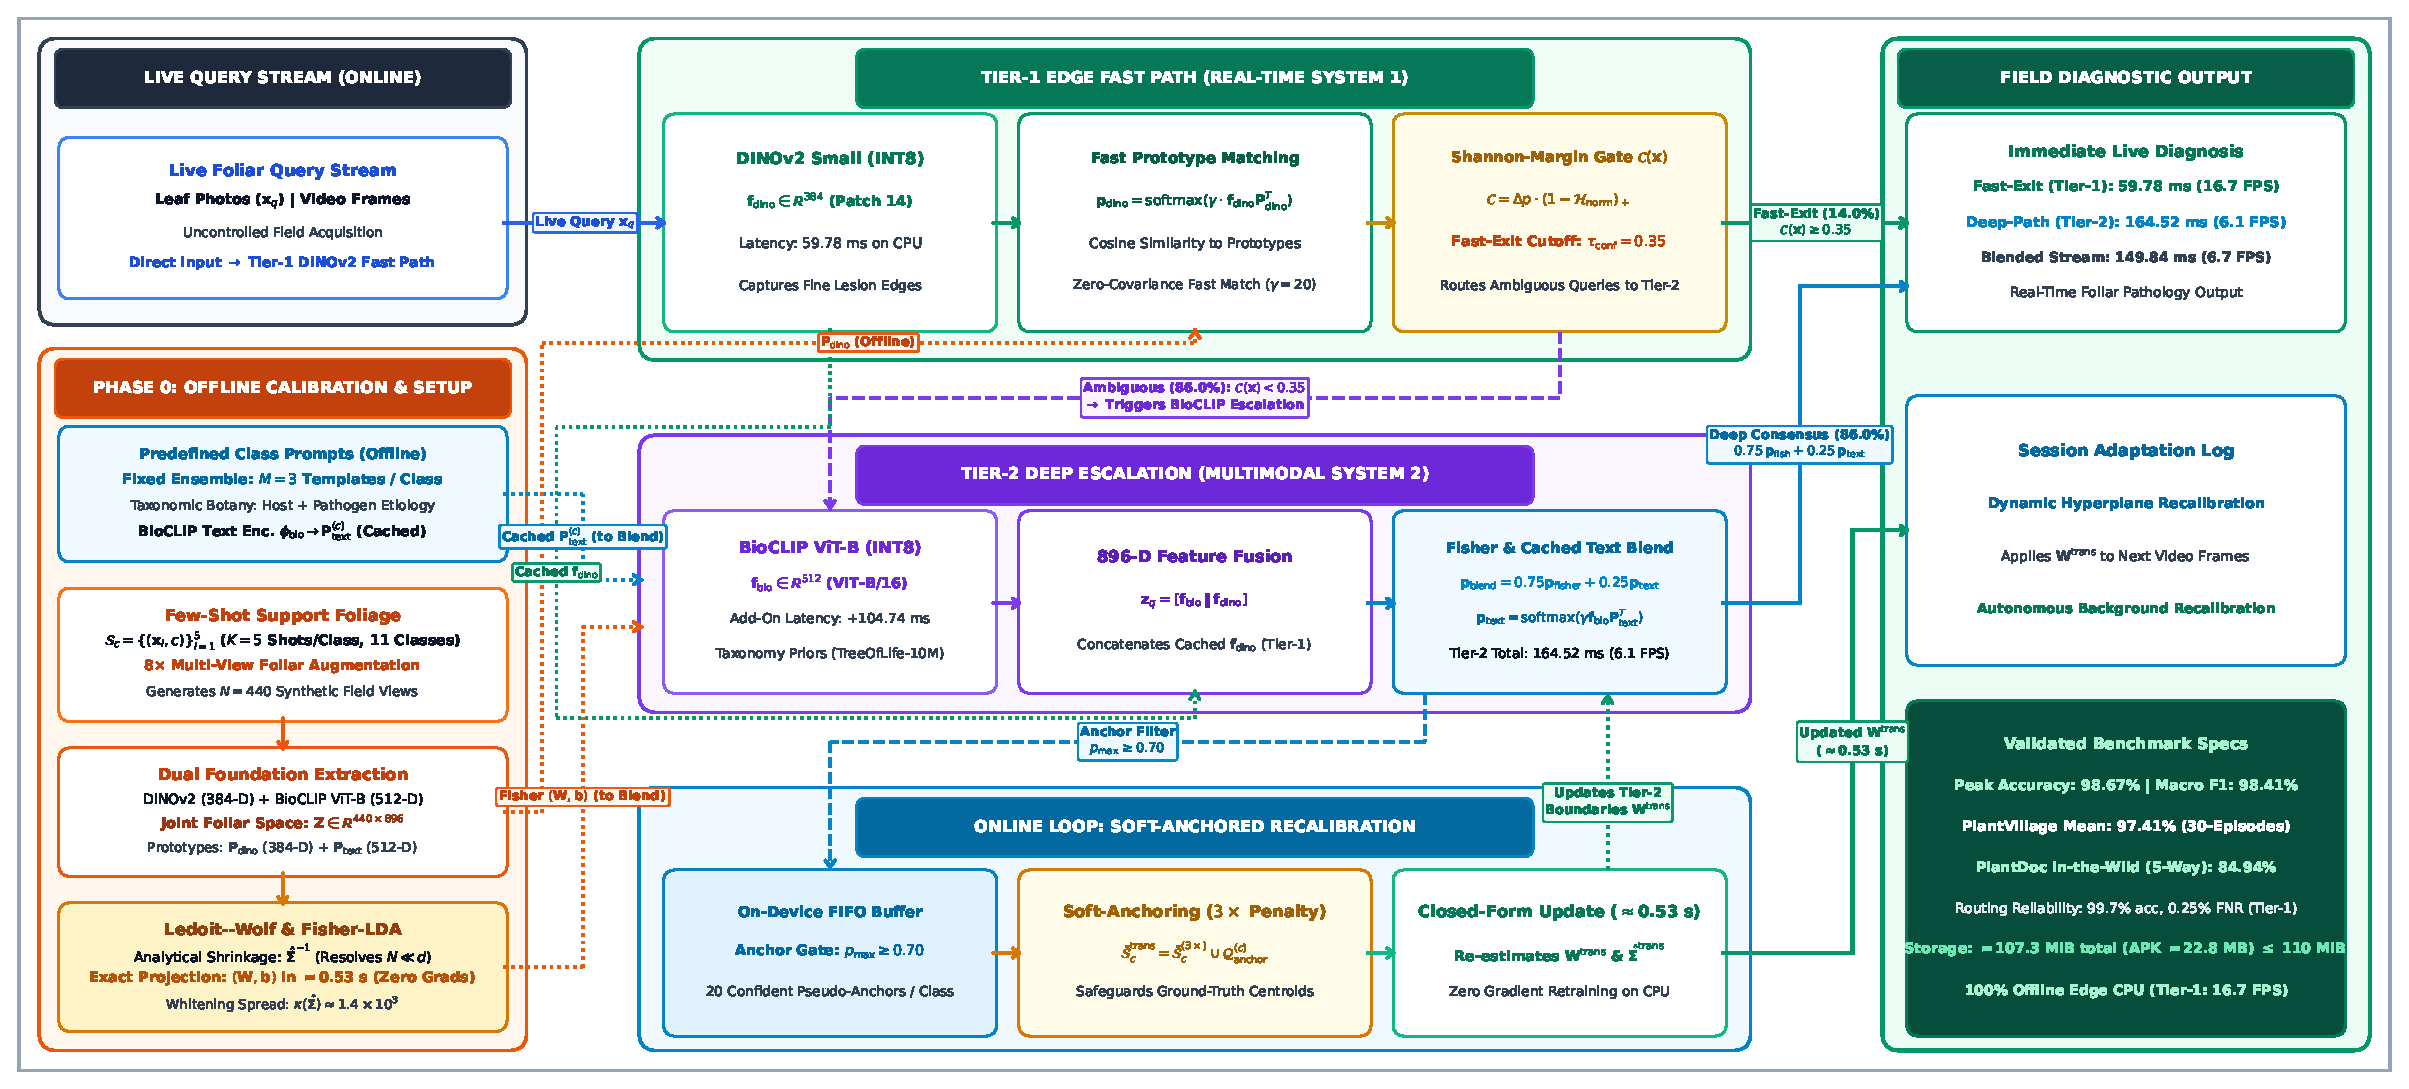
\includegraphics[width=0.88\textwidth]{fig_architecture.pdf}
\caption{Architecture of BioDINO-Edge. Phase~0 (offline) computes Tier-1 visual prototypes and closed-form Fisher-LDA projections while caching botanical text prototypes. During inference, the Shannon-margin uncertainty gate sends routine foliage through Tier-1 fast prototype matching (DINOv2) and escalates ambiguous queries to Tier-2 multimodal consensus (BioCLIP), followed by closed-form soft-anchored transductive recalibration.}
\label{fig:architecture}
\end{figure*}

\subsection{Dual-Foundation Foliar Representation}
\label{sec:feature_extraction}
BioDINO-Edge couples two frozen backbones. DINOv2 provides patch-level features of leaf surface texture and lesion boundaries, while BioCLIP provides organismal taxonomic priors. Concatenating their $\ell_2$-normalized outputs yields an 896-dimensional descriptor that encodes localized symptoms alongside host context.

\subsubsection{Few-Shot Multi-View Support Augmentation}
To overcome covariance ill-conditioning when reference data are scarce ($K = 5$), each support leaf $\mathbf{x} \in \mathcal{S}_c$ is resized to $224 \times 224$ pixels, normalized, and passed through an 8-view stochastic augmentation pipeline approximating field variations. The pipeline applies random horizontal and vertical flips, rotations within $\pm 15^\circ$, and color jitter (brightness, contrast, and saturation factors of $0.2$). Generating eight views per leaf yields $|\tilde{\mathcal{S}}_c| = 8K = 40$ augmented views per class, producing $N = 40C = 440$ total support representations for $C = 11$. This expansion brings the support sample size close to half the joint feature dimension ($d/2 = 448$), which stabilizes the covariance condition number. Although augmented views are not strictly independent, regularized shrinkage prevents numerical degeneracy and guarantees positive-definiteness. For the controlled PlantVillage comparison we use the cached single-view features; Table~\ref{tab:aug_sensitivity} isolates the 8-view expansion. PlantDoc results use the 8-view features throughout.

\subsubsection{Dual-Foundation Embedding Fusion}
Each augmented view $\tilde{\mathbf{x}} \in \tilde{\mathcal{S}}_c$ is passed through the frozen backbones. DINOv2 ViT-S/14 (patch size 14, 384-D)~\cite{oquab2023dinov2} and BioCLIP ViT-B/16~\cite{stevens2024bioclip} extract $\ell_2$-normalized feature vectors:
\begin{equation}
    \mathbf{f}_{\text{dino}} = \frac{\phi_{\text{dino}}(\tilde{\mathbf{x}})}{\|\phi_{\text{dino}}(\tilde{\mathbf{x}})\|_2} \in \mathbb{R}^{384}, \qquad
    \mathbf{f}_{\text{bio}} = \frac{\phi_{\text{bio}}(\tilde{\mathbf{x}})}{\|\phi_{\text{bio}}(\tilde{\mathbf{x}})\|_2} \in \mathbb{R}^{512}.
\end{equation}
Concatenating the two normalized embeddings yields the 896-dimensional joint descriptor:
\begin{equation}
    \mathbf{z} = [\mathbf{f}_{\text{bio}} \,\|\, \mathbf{f}_{\text{dino}}] \in \mathbb{R}^{896}.
\end{equation}
Visual prototypes for the Tier-1 classifier are computed as the normalized mean of the support views:
\begin{equation}
    \mathbf{P}_{\text{dino}}^{(c)} = \text{Normalize}\left(\frac{1}{|\tilde{\mathcal{S}}_c|}\sum_{\tilde{\mathbf{x}} \in \tilde{\mathcal{S}}_c} \mathbf{f}_{\text{dino}}(\tilde{\mathbf{x}})\right),
\end{equation}
yielding the Tier-1 visual prototype matrix $\mathbf{P}_{\text{dino}} \in \mathbb{R}^{C \times 384}$.

\subsubsection{Botanical Taxonomic Prompts and Negation Avoidance}
BioCLIP provides a shared vision--language space, but running text decoders on device costs latency and memory. We therefore define $M = 3$ botanical prompt templates $\{T_c^{(m)}\}_{m=1}^M$ offline for each disease class $c \in \{1, \dots, C\}$. Each template covers three elements:
\begin{enumerate}
    \item \textbf{Host species:} Botanical genus and species (e.g., \textit{Malus domestica}, \textit{Vitis vinifera}, \textit{Solanum tuberosum}).
    \item \textbf{Pathogen name:} Scientific name of the causal agent (e.g., \textit{Venturia inaequalis}, \textit{Guignardia bidwellii}, \textit{Phytophthora infestans}).
    \item \textbf{Visible symptoms:} Diagnostic foliar symptoms (e.g., ``olive-green velvety lesions'', ``tiger-stripe interveinal chlorosis'', ``target-board concentric rings'').
\end{enumerate}
Syntactic negations such as ``healthy leaf without lesions'' or ``no necrotic spots'' are excluded. Vision--language models handle negation poorly~\cite{alhamoud2025vision}, consistent with their bag-of-words, order-insensitive behaviour~\cite{yuksekgonul2023when}: a negated healthy description is encoded close to the disease concepts it mentions rather than away from them. With the BioCLIP text encoder, the three healthy prototypes lie at a mean cosine similarity of 0.557 to the eight disease prototypes when described by negation (range 0.422--0.666), against 0.483 (range 0.359--0.633) for purely positive histological descriptions (``clean vibrant green lamina with smooth intact blade surface''). The same pattern appears end to end: switching the three healthy classes to negated prompts raises transductive FNR from 1.25\% to 2.57\% on the prompt-ablation split. Omitting negations therefore keeps healthy prototypes out of disease clusters and lowers false-negative escape, so every template describes healthy tissue with affirmative terms (e.g., ``clean green foliage'', ``intact smooth leaf lamina'').

During Phase~0, BioCLIP's text encoder $\phi_{\text{bio,txt}}(\cdot)$ encodes each prompt ensemble, and the results are averaged and $\ell_2$-normalized:
\begin{equation}
    \mathbf{P}_{\text{text}}^{(c)} = \text{Normalize}\left(\frac{1}{M}\sum_{m=1}^M \phi_{\text{bio,txt}}(T_c^{(m)})\right) \in \mathbb{R}^{512}.
\end{equation}
The resulting matrix $\mathbf{P}_{\text{text}} \in \mathbb{R}^{C \times 512}$ is cached on device, so there is no runtime tokenization or language-model overhead.

\subsection{Closed-Form Analytical Adaptation via Regularized Fisher-LDA}
\label{sec:fisher_adaptation}

\subsubsection{Multiclass Fisher Linear Discriminant Formulation}
Standard nearest-centroid and cosine-similarity classifiers implicitly assume uniform variance across all feature directions ($\mathbf{\Sigma} = \mathbf{I}$). That assumption does not hold for leaves: shared vegetative structure (such as venation and lamina) creates high-variance directions that mask lesion differences between diseases on the same host. Multiclass Fisher Linear Discriminant Analysis (Fisher-LDA)~\cite{fisher1936use, rao1948utilization} resolves this by weighting features by $\hat{\mathbf{\Sigma}}^{-1}$, which down-weights those shared directions and amplifies low-variance directions containing discriminative lesion symptoms.

Fisher-LDA computes a linear projection matrix $\mathbf{W} \in \mathbb{R}^{C \times d}$ and bias vector $\mathbf{b} \in \mathbb{R}^C$ that maximize between-class scatter $\mathbf{S}_B$ relative to within-class scatter $\mathbf{S}_W$:
\begin{equation}
    \label{eq:fisher_weights}
    \mathbf{W} = [\boldsymbol{\mu}_1, \dots, \boldsymbol{\mu}_C]^T \hat{\mathbf{\Sigma}}^{-1}, \qquad
    b_c = -\frac{1}{2}\boldsymbol{\mu}_c^T \hat{\mathbf{\Sigma}}^{-1}\boldsymbol{\mu}_c - \log C,
\end{equation}
where $\hat{\mathbf{\Sigma}}$ is the regularized pooled within-class covariance matrix ($d = 896$) and class priors are uniform ($\pi_c = 1/C$).

\subsubsection{Small-Sample Singularity \texorpdfstring{($N \ll d$)}{(N << d)}}
Evaluating Eq.~\eqref{eq:fisher_weights} requires inverting the empirical pooled within-class scatter matrix over all $C = 11$ classes:
\begin{equation}
    \label{eq:within_class_scatter}
    \mathbf{S}_W = \frac{1}{N-C}\sum_{c=1}^C \sum_{\mathbf{z} \in \tilde{\mathcal{S}}_c} (\mathbf{z}-\boldsymbol{\mu}_c)(\mathbf{z}-\boldsymbol{\mu}_c)^T \in \mathbb{R}^{d \times d}.
\end{equation}
With $N = 440$ support representations and $d = 896$ features, the support size is far below the feature dimension ($N \ll d$), and the same holds after estimating class means. Here $N - C = 440 - 11 = 429$ is the degrees of freedom left, so the rank of $\mathbf{S}_W$ is bounded:
\begin{equation}
    \label{eq:rank_bound}
    \text{rank}(\mathbf{S}_W) \le \min(d, N-C) = 429 < 896.
\end{equation}
Hence, $\mathbf{S}_W$ has a nullity of at least $896 - 429 = 467$: at least 467 of its eigenvalues are zero ($\det(\mathbf{S}_W) = 0$), and it cannot be inverted directly.

\subsubsection{Analytical Ledoit--Wolf Covariance Shrinkage}
\label{sec:shrinkage}
To restore invertibility without manual hyperparameter tuning (such as searching over a grid of ridge penalties $\mathbf{S}_W + \epsilon \mathbf{I}$), we apply analytical Ledoit--Wolf shrinkage~\cite{ledoit2004well}, which contracts $\mathbf{S}_W$ toward a spherical target $\nu \mathbf{I}_d$:
\begin{equation}
    \hat{\mathbf{\Sigma}} = (1 - \rho^*)\mathbf{S}_W + \rho^* \nu \mathbf{I}_d, \qquad \nu = \frac{1}{d}\text{Tr}(\mathbf{S}_W).
    \label{eq:lw_target}
\end{equation}
The optimal shrinkage intensity $\rho^* \in (0, 1]$ is determined in closed form by minimizing expected quadratic Frobenius risk:
\begin{equation}
    \rho^* = \min\left(1, \frac{\sum_{i=1}^N \|(\mathbf{z}_i - \boldsymbol{\mu}_{c_i})(\mathbf{z}_i - \boldsymbol{\mu}_{c_i})^T - \mathbf{S}_W\|_F^2}{N^2 \left[\text{Tr}(\mathbf{S}_W^2) - \frac{1}{d}\text{Tr}^2(\mathbf{S}_W)\right]}\right).
    \label{eq:lw_shrinkage}
\end{equation}
This shifts zero eigenvalues to positive values $\tilde{\lambda}_i = (1 - \rho^*)\lambda_i + \rho^* \nu \ge \rho^* \nu > 0$, ensuring that $\hat{\mathbf{\Sigma}}$ is strictly positive-definite and invertible. Its inverse $\hat{\mathbf{\Sigma}}^{-1}$ is solved stably via Cholesky decomposition ($\hat{\mathbf{\Sigma}} = \mathbf{L}\mathbf{L}^T$). Scoring a query $\mathbf{z}$ as $\mathbf{l}_{\text{fisher}} = \mathbf{z}\mathbf{W}^T + \mathbf{b}$ then requires only $C \cdot d$ multiply-accumulate (MAC) operations ($9{,}856$ MACs for $C=11$), requiring minimal on-device computation.

Weighting by $\hat{\mathbf{\Sigma}}^{-1}$ acts as a whitening transform: each eigen-direction with variance $\lambda_i$ is rescaled by $1/\lambda_i$, dampening common leaf morphology while highlighting subtle lesion variations. The condition number
\begin{equation}
    \kappa(\hat{\mathbf{\Sigma}}) = \lambda_{\max}(\hat{\mathbf{\Sigma}}) / \lambda_{\min}(\hat{\mathbf{\Sigma}})
    \label{eq:whitening_spread}
\end{equation}
reflects the dynamic range of this feature rescaling. Because the augmented support views are formed from real leaves, shrinkage guarantees numerical stability across all sample sizes.

\subsection{Adaptive Two-Tier Classification and Edge Deployment}
\label{sec:edge_cascade}

\subsubsection{Tier-1 Fast Path and Shannon Uncertainty Gating}
For an incoming leaf image $\mathbf{x}$, Tier~1 extracts the normalized DINOv2 embedding $\mathbf{f}_{\text{dino}} \in \mathbb{R}^{384}$ and computes fast prototype logits by temperature-scaled cosine similarity against the visual prototypes $\mathbf{P}_{\text{dino}} \in \mathbb{R}^{C \times 384}$:
\begin{equation}
    \label{eq:tier1_logits}
    \mathbf{l}_{\text{dino}} = \gamma \cdot \left(\mathbf{f}_{\text{dino}} \mathbf{P}_{\text{dino}}^T\right), \qquad \gamma = 20.0.
\end{equation}
A softmax yields the fast posterior probabilities:
\begin{equation}
    \label{eq:tier1_softmax}
    \mathbf{p}_{\text{dino}} = \text{softmax}(\mathbf{l}_{\text{dino}}) \in \Delta^{C-1}.
\end{equation}
Tier~1 uses cosine prototype matching only, with no covariance projection, so the Fisher-LDA computation is spent only on queries that need it. The Tier-1 prediction is $\hat{y}_{\text{tier1}} = \arg\max_c p_{\text{dino}, c}$.

Certainty is scored from the same forward pass, so no extra computation is needed. We combine the top-2 margin and normalized entropy into a confidence score $\mathcal{C}(\mathbf{x}) \in [0, 1]$:
\begin{equation}
    \label{eq:shannon_gate}
    \mathcal{C}(\mathbf{x}) = \left(p_{\text{dino}, (1)} - p_{\text{dino}, (2)}\right) \cdot \left(1.0 - \mathcal{H}_{\text{norm}}(\mathbf{x})\right)_+,
\end{equation}
where $p_{\text{dino}, (1)}$ and $p_{\text{dino}, (2)}$ are the top-1 and top-2 posteriors, $(\cdot)_+ = \max(0, \cdot)$, and $\mathcal{H}_{\text{norm}}(\mathbf{x})$ is the normalized Shannon entropy~\cite{shannon1948mathematical}:
\begin{equation}
    \mathcal{H}_{\text{norm}}(\mathbf{x}) = -\frac{1}{\log C}\sum_{c=1}^C p_{\text{dino}, c}\log(p_{\text{dino}, c} + \epsilon),
\end{equation}
with $\epsilon = 10^{-12}$ for numerical stability. The rectifier $(\cdot)_+$ simply guards against floating-point round-off. Ambiguous queries with near-uniform posteriors exhibit high entropy ($\mathcal{H}_{\text{norm}} \to 1$) and negligible margin, driving $\mathcal{C}(\mathbf{x}) \to 0$. When $\mathcal{C}(\mathbf{x}) \ge \tau_{\text{conf}}$ ($\tau_{\text{conf}} = 0.35$, calibrated on validation data), Tier~1 accepts the prediction; otherwise, the query escalates to Tier~2.

\subsubsection{Tier-2 Multimodal Consensus Escalation}
When $\mathcal{C}(\mathbf{x}) < \tau_{\text{conf}}$, the query goes to Tier~2. BioCLIP ViT-B extracts $\mathbf{f}_{\text{bio}} \in \mathbb{R}^{512}$, which is concatenated with the Tier-1 embedding to form $\mathbf{z} = [\mathbf{f}_{\text{bio}} \,\|\, \mathbf{f}_{\text{dino}}] \in \mathbb{R}^{896}$. Two posteriors are then computed: the discriminant visual posterior $\mathbf{p}_{\text{fisher}} = \text{softmax}(\mathbf{z}\mathbf{W}^T + \mathbf{b})$ and the taxonomic text posterior $\mathbf{p}_{\text{text}} = \text{softmax}(\gamma \cdot \mathbf{f}_{\text{bio}}\mathbf{P}_{\text{text}}^T)$. These are fused with Fisher consensus weight $w_{\text{lda}} = 0.75$:
\begin{equation}
    \label{eq:multimodal_blend}
    \mathbf{p}_{\text{blend}} = w_{\text{lda}} \, \mathbf{p}_{\text{fisher}} + (1 - w_{\text{lda}}) \, \mathbf{p}_{\text{text}},
\end{equation}
and the final diagnosis is $\hat{y} = \arg\max_c p_{\text{blend}, c}$.

\subsubsection{Soft-Anchored Transductive Recalibration}
\label{sec:transductive}
In 5-shot calibration, each centroid $\boldsymbol{\mu}_c$ is estimated from only five support leaves. Lighting changes, shadows, and symptom progression can shift prototypes between support images and field queries. To adapt without manual labels, confident Tier-2 queries ($\max_c p_{\text{blend}, c} \ge 0.70$) are buffered into a first-in, first-out (FIFO) queue as reference anchors $\mathcal{Q}_{\text{anchor}}^{(c)}$, limited to 20 anchors per class. Verified support samples receive a $3\times$ weight factor so that pseudo-label drift does not shift class centroids away from confirmed disease definitions:
\begin{equation}
    \label{eq:transductive_set}
    \tilde{\mathcal{S}}_c^{\text{trans}} = \tilde{\mathcal{S}}_c^{(3\times)} \cup \mathcal{Q}_{\text{anchor}}^{(c)}.
\end{equation}
Once the buffer fills during scouting, centroids $\boldsymbol{\mu}_c^{\text{trans}}$ and pooled scatter matrix $\mathbf{S}_W^{\text{trans}}$ are re-estimated, the shrinkage parameter $\rho^*$ is recomputed, and updated projection parameters $(\mathbf{W}^{\text{trans}}, \mathbf{b}^{\text{trans}})$ are resolved via Cholesky substitution in about 0.53\,s. This runs asynchronously in the background, so Tier~1 keeps operating with static prototypes while later Tier-2 decisions use the updated ones.

Three design choices keep this update stable and efficient. First, the 0.70 confidence threshold ensures high pseudo-label purity ($\approx$98\%) while avoiding the coverage starvation that collapses accuracy at higher thresholds ($\ge$0.80). Second, the support weight anchors class centroids against manifold drift: the original support leaves are repeated $w_{\mathrm{sup}}$ times so that in the re-estimated centroid
$\boldsymbol{\mu}_c^{\text{trans}} = (w_{\mathrm{sup}}\sum_{\mathbf{x}\in\mathcal{S}_c}\mathbf{x} + \sum_{\mathbf{q}\in\mathcal{Q}_{\text{anchor}}^{(c)}}\mathbf{q}) / (w_{\mathrm{sup}}|\mathcal{S}_c| + |\mathcal{Q}_{\text{anchor}}^{(c)}|)$
the verified leaves outvote pseudo-labels, and $w_{\mathrm{sup}}$ is set per deployment rather than fixed globally. With five support leaves per class and up to twenty anchors, $w_{\mathrm{sup}}=3$ keeps a single support leaf worth roughly one and a half confident anchors on the 11-class benchmark, whereas the field protocol, which draws only two anchors per class, uses $w_{\mathrm{sup}}=1$ or $2$ and no confidence threshold because a fixed threshold there leaves too few eligible anchors. Third, the 20-anchor cap bounds update latency while preventing frequent classes from introducing sample imbalance.

\subsection{Two-Tier Quantized Edge Model Packaging and Android Architecture}
\label{sec:packaging}
Agricultural edge devices operate under limited memory and power budgets, and field connectivity is often unreliable~\cite{sharif2026real,radocaj2025evolution}. BioDINO-Edge therefore never sends a diagnosis over the network: once installed, every query is processed on device without streaming, cloud offloading, or server calls. The framework is partitioned into two INT8-quantized Open Neural Network Exchange (ONNX) binaries (footprints reported in mebibytes (MiB), where $1\,\text{MiB} = 2^{20}$ bytes), separating a fast standalone engine from an on-demand deep companion.

\textbf{Tier 1 Standalone Engine} (\path{biodino_mobile_int8.onnx}): Packaged inside an APK (occupying $\approx$22.8\,MB on device, where the base model binary accounts for $\approx$22.0\,MiB on disk and $\approx$15.1\,MiB deflated). It integrates the DINOv2 Small INT8 backbone, calibrated Phase~0 prototypes, and the Shannon confidence gate executed via the ONNX Runtime C++ execution provider. Installing the APK enables immediate offline diagnosis.

\textbf{Tier 2 Companion Module} (\path{biodino_companion_int8.onnx}): The companion engine occupies $\approx$85.3\,MiB on disk, containing the BioCLIP ViT-B INT8 backbone and the 896-dimensional Fisher projection matrix. It is fetched on-demand when high-precision multimodal escalation is requested, functioning completely offline once stored.

Together, both binaries occupy $\approx$107.3\,MiB of flash storage on device.

\textbf{On-Device Few-Shot Pathogen Enrollment.} To accommodate field scenarios where agronomists encounter novel or uncataloged foliar pathologies, the Android application integrates an interactive on-device enrollment interface. Users can register a new disease class directly in the field by capturing 1--5 exemplar photos of symptomatic foliage, along with an optional healthy leaf reference from the same host crop. Upon capture, the application extracts foundation embeddings, runs on-device multi-view augmentation, and resolves the regularized discriminant projection via EJML Cholesky factorization in sub-second time, enabling immediate subsequent detection entirely offline without network connectivity.

% =============================================================================
